\documentclass[11pt]{article}
\usepackage{acl2015}
\usepackage{times}
\usepackage{url}
\usepackage{latexsym}
\usepackage{acl2015}
\usepackage{relsize}
\usepackage{hyperref}
\usepackage{float}
\usepackage{lipsum}
\usepackage{booktabs,chemformula}
\usepackage{blindtext}
%\textunderscore
%\setlength\titlebox{5cm}\
\usepackage{graphicx}
\graphicspath{ {./images/} } 

\title{BERT-Based Emotion Recognition\\[0.2em]\smaller{}Team Gold}
\author{
  Aiman Haider \\\And
  Maobin Guo \\\And
  Pranav Manjunath \\\And
  Xinyi Pan}

\date{}

\pagenumbering{alph}

\begin{document}
\maketitle

\begin{abstract}
Multi-class Emotion Detection in Text has been a conventionally difficult task given the presence of subjectivity, subtleties and stylizations used in text. While a number of conventional and deep learning techniques have been used, the project found the BERT Model to be the best performing so far, and developed an application to classify text from an external dataset into the seven basic emotion classes.
\end{abstract}

\section{Introduction}

Understanding another person’s emotions is critical in interpersonal communication. Discussion on emotions has a long history and has become more popular in contemporary business scenarios. Since Greek and Roman times~\cite{affect_rw1}, decision-makers utilized public opinion to advocate their policies and formed democracies. Nowadays, public opinion and emotions are more significant not only in politics but also valuable for product reviews and promotion~\cite{affect_rw2}. The proliferation of online activities and the exponential growth of information on the internet endow industry and academia with the capacity for affective computing~\cite{affect_rw1}, which is the capacity for recognizing, inferring, and deciphering human emotion. Affective computing serves an increasingly central role in spam detection technology, recommendation systems, and most importantly, business intelligence, where the corporate interest lies~\cite{affect_rw2}.  

% our work & outline to be added here
In this project, we aim to explore the domain of affective computing by performing multi-class classification of emotions by comparing different machine learning algorithms, ranging from logistic regression, LSTM, to BERT. We first review relevant literature in Section~\ref{sec:background}. The methodologies adopted are then explained in Section~\ref{sec:method}, and the results are discussed in Section~\ref{sec:result}. We also developed an interactive application on unlabeled Facebook Comments with Python, which is shown in Section~\ref{sec:app}.

\section{Background}
\label{sec:background}

Affective computing which deals with identification, processing, interpretation, and simulation of human emotional states intelligently from data~\cite{affect_rw1}, consists of sentiment analysis and emotion recognition. Though there are close similarities between sentiments and emotions, the subtleties between these two subjective terms also exist~\cite{affect_rw3}. Sentiments are more stable and targeted while emotions are short-lived and transient. Accordingly, the mining and analysis of sentiments and emotions are semantically distinct from each other. 

In addition, sentiment analysis and emotion recognition have different levels of granularity~\cite{affect_rw1}. The former is characterized as coarse-grained affect recognition since it performs a binary classification task in general with outputs such as positive versus negative~\cite{affect_rw1},~\cite{affect_rw2}. In contrast, the latter is referred to as fine-grained affect recognition~\cite{affect_rw1},~\cite{affect_rw2} as it is based on a larger set of emotion labels including happiness, sadness, anger, and surprise~\cite{affect_rw6}. 

In light of the similarity between detecting coarse-grained and fine-grained emotions, approaches to emotion recognition can be mainly categorized into lexicon-based techniques and statistical methods~\cite{affect_rw2}. The lexicon-based approach, also commonly referred to as a knowledge-based approach~\cite{affect_rw2}, exploits the lexical, morphological, and syntactic characteristics of texts to perform text-based emotion recognition. Extensive literature has proposed, evaluated, and leveraged lexicon-based techniques such as WordNet-Affect~\cite{affect_rw8}, SentiWordNet~\cite{affect_rw9}, and SenticNet~\cite{affect_rw10} in the last two decades. Nonetheless, Cambria~\cite{affect_rw2} states that the lexicon-based approach is weak when the mining and detection of emotions are involved with linguistic rules. Moreover, emotion recognition with knowledge-based techniques highly relies on human-generated baselines, such as a comprehensive corpus annotated by humans. However, given that the original intention of humans to explore this approach is to enable machines to detect emotions automatically, knowledge-based techniques are becoming obsolete, and therefore scholars have proposed and increasingly adopted another category of methodologies viz. statistical methods~\cite{affect_rw1},~\cite{affect_rw2}. 

Among these,  there has been a special focus on supervised machine learning techniques~\cite{affect_rw1}, including Naive Bayes, Maximum Entropy, and Support Vector Machines~\cite{affect_rw11}. Deep learning, an unsupervised machine learning technique, is also widely exploited in the existing literature of emotion recognition~\cite{affect_rw1}. One of the advantages of statistical methods is that it provides more accurate and reasonable classification compared to knowledge-based approaches. For instance, Pang et al. ~\cite{affect_rw11} found that supervised machine learning techniques significantly outperform knowledge-based techniques in terms of classification accuracy. Also, statistical approaches have been found more powerful than other alternatives in predicting lexical affinity between words and the frequency of word co-occurrence~\cite{affect_rw2}. This report, too, adopts the deep learning approach to the task of emotional  classification.

% machine learning-link to our project

\section{Methodology}
\label{sec:method}

A few techniques are explored first to understand their performances and appropriateness, and then an application is developed using the BERT model, which showed the best results.

The dataset used is a dataset collected by the International Survey on Emotion Antecedents and Reactions (ISEAR) during the 1990s. For building the ISEAR, 1,096 participants who have different cultural backgrounds completed questionnaires about experiences and reactions for seven emotions including anger, disgust, fear, joy, sadness, shame, and guilt, 7 major emotion classes on which our study is based~\footnote{\url{https://www.unige.ch/cisa/research/materials-and-online-research/research-material/}}. This dataset consists of 7,666 sentences from around 3000 respondents in 37 countries on all 5 continents. Extensive literature has evaluated this dataset for emotion recognition and achieved impressive performance. Therefore, we decided to utilize this dataset for our classification purpose. The dataset is split into 75\% for training and 25\% for testing. 

\subsection{Multinomial Logistic Regression}

Given the task of multinomial classification of emotions, the first method applied is multinomial logistic regression, which is a standard supervised machine learning algorithm for the classification of more than two classes~\cite{textbook}. The emotions are classified by evaluating the probability of the text to belong to each potential emotional class. During this process, one emotion class is chosen as the baseline category. The multinomial logistic model is therefore a set of logistic regression models for each emotional class, compared to this baseline.

A model is built using the multinomial logistic regression on TF-IDF representations (features) of the text in the dataset and it is found that it has an overall accuracy was 55\% across all emotion labels.

\subsection{Long Short Term Memory and Bidirectional Long Short Term Memory}
\label{sect:BiLSTM}

Next, we attempt two popular methods in Deep Learning - LSTM and BiLSTM, which stands for Long Short Term Memory and Bidirectional Long Short Term Memory. The LSTM is a special type of Recurrent Neural Network (RNN), which  “remembers” and uses immediate previous values through feedback loops, that can learn long term patterns based on a combination of immediate and some old retained memory as can be seen through its architecture as in the figure~\ref{fig:bt}.

\begin{figure}
\caption{Structure of BiLSTM}
\label{fig:bt}
\centering
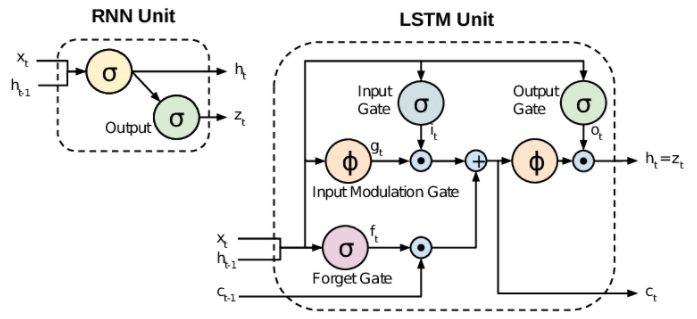
\includegraphics[scale=0.4]{images/BiLSTM.png}
\end{figure}

First, we try using LSTM with GLove Embeddings on the dataset. The text is preprocessed by casing, tokenization, and lemmatization and then vectorized using the dictionary entered by the pre-trained GLove vector model~\cite{glove} which gives us the corresponding Embedding Vectors. Next, it is encoded with LSTM and then passed through a softmax layer for classification. Next, we try using the BiLSTM, which is a variant of LSTM that processes the information in dual ways across the starting and terminating neurons of the network for faster training and better flow of information. It is a sequence processing model that consists of two LSTMs where one takes the input in a forward direction, and the other in the backward direction. Due to this, BiLSTM increases the amount of information available to the network, improving the context available to the algorithm. It is surprising, however, that both give similar and much lower accuracy of 40.9\%. This could possibly be due to the equal focus on all tokens, which hinders the model from capturing the important words/features as well as in ~\ref{sec:method}.

\subsection{Bidirectional Encoder Representations from Transformers}
\label{ssec:BERT}

We then turn to BERT, short for Bidirectional Encoder Representations from Transformers. BERT is a state-of-the-art pre-training language representation. It is based on the transformer framework where the input text sequence is deeply represented by encoding and decoding~\cite{devlin2018bert} and uses a multi-head self-attention mechanism~\cite{li2019exploiting}. The attention mechanism extracts the different "role" information in word representations, namely $Q$ (Query), $K$ (Key), and $V$ (Value). The attention weight is obtained by scaling the dot product of the $Q$ of the current word and the $K$ of the word being noticed and then obtained by the softmax layer. The attention weight is assigned to the $V$ of the current word and then added to its representation. BERT uses Masked LM (Masked Language Model) for training. These allow for a few words in the token sequence (sentence) to be masked and facilitate its prediction as also in predicting the next "sentence". The goal of Masked LM ensures that BERT can obtain a representation of the target word that combines left and right bidirectional context information. 

BERT mainly functions to obtain a representation of a sentence (word sequence), which is expected to reflect the relationship between words. To this end, it has designed additional tags that indicate the beginning, end, and connection of the word sub-sequence; and the position information of the word is also added during the processing. The real words, symbols, marks, and segmented units, are referred to as tokens. As shown in~\ref{fig:bert}, the pre-training input of BERT is embedded by token Entry (token Embeddings), segment embeddings (Segment Embeddings), and position embedding (Position Embeddings). These then go through the layers of encoders.

\begin{figure}
\label{fig:bert}
\caption{Structure of BERT}
\centering
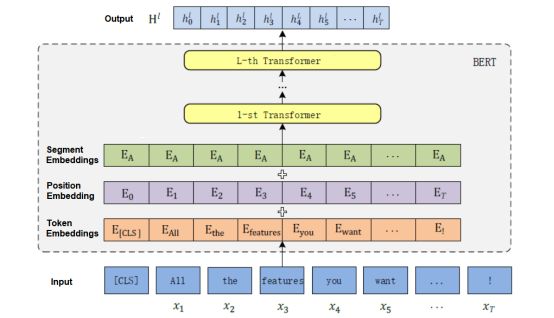
\includegraphics[scale=0.5]{images/BERT.png}
\end{figure}

Let L be the number of BERT layers, \textit{dimh} represents the dimension of the word, Transformerl represents the mapping of l layer \(\left ( l = 1, 2, \cdots , L \right )\) determined by Transformer, \(x = \left ( x_{1}, x_{2}, \cdots , x_{T}  \right )\) is a text input to BERT, and \(H^{l} = \left ( h_{1}^{l}, h_{2}^{l}, \cdots, h_{T}^{l} \right )\) are recorded as the output of the $l^{th}$ layer. Hence, $H_{l} = Transformerl\left ( H_{l}-1\right )$. Finally, the output of BERT is $H^{L} = \left ( h_{1}^{L}, h_{2}^{L}, \cdots, h_{T}^{]} \right )$. 

Google provides two pre-trained versions of the BERT model: BERT\_BASE (L=12, H=768, A=12, Total Parameters=110M) and BERT\_LARGE (L=24, H=1024, A=16, Total Parameters=340M) where L represents the number of layers (Transformer Blocks), H represents the space dimension, A represents the number of attention heads, and Total Parameters represents the number of parameters. We use the BERT\_BASE version on the datset and find it to be the best performing among the ones considered. We also compared this to the baseline results for the data and find that it outperformed those results as well by a slight margin.


\section{Results}
\label{sec:result}

As is mentioned above, the BERT model performs better than the others considered. The results for the BERT model on the dataset can be seen in Table ~\ref{tab:modelpre}. The Attention mechanism seems to be a major reason for this as it does not distribute the weightage of each embedding equally, rather focuses on the important ones.

%\begin{table}[ht]
\begin{table}[h]
    \centering
    \begin{tabular}{lllll}
    \toprule
    Emotion & Precision & Recall & F1-Score \\
    \midrule
    Disgust  & 0.70 & 0.69 &  0.70 \\   
    Fear  & 0.77 & 0.77 &  0.77 \\
    Shame  & 0.59 & 0.51 &  0.55 \\
    Guilt  & 0.62 & 0.64 &  0.63 \\
    Anger  & 0.60 & 0.59 &  0.59 \\
    Sadness  & 0.71 & 0.73 &  0.72 \\
    Joy  & 0.81 & 0.90 &  0.85 \\
    \midrule
    Accuracy & \multicolumn{3}{c}{0.69} \\
    Macro avg & 0.69 & 0.69 & 0.69 \\
    Weighted avg & 0.69 & 0.69 & 0.69
    \bottomrule
    \end{tabular}
    \caption{Output of BERT}
    \label{tab:modelpre}
\end{table}
%\Blindtext\Blindtext

The model reports an overall accuracy of 69\% with a macro F1, Recall and Precision of 0.69. This model, thus, also seems to indicate a good balance of sensitivity and specificity overall. Also, it should be pointed out that its results have been pretty close to that best metrics reported for the dataset which is 67\%. ~\footnote{\url{https://arxiv.org/pdf/1908.01587.pdf}}		

\newline
Further, it can be seen that the model has a much better performance when it comes to predicting joy than other emotions. It can be seen that shame, anger and the upsetting emotions do not fare as well as joy related sentences. This can possibly be because of the preponderance of a variety of "upset" emotions which may have made it difficult for the model to capture the subtleties that well. Besides, the limitations due to linguistic subjectivity and stylizations are other possible reasons. Nonetheless, it performs well on these parameters when compared to afore-mentioned models. This is evident through its better-performing confusion matrix, too. 

\section{Application}
\label{sec:app} 

To practically demonstrate, a Python application is built using the Tkinter library in Python and ran on unlabeled Facebook Comments from Kaggle. The application fetches random comments from Kaggle, sends it through the ISEAR-trained BERT model and displays the predicted emotion along with the comment. The application uses the sample Panda images found on Powtoon and associates each emotion to a respective Panda Emoji. Figures in the appendix show three sample screenshots from the application. 
 

\section{Conclusions}
\label{sec:con}

While a number of statistical methods are being increasingly used to class text into emotions, the project found the BERT model to be the most efficient. It found that because of its unique architecture, it can generally identify important words of a sentence that render it emotion. However, the presence of subjectivity and transient nature of emotions still remains a limitation that should addressed in future works.

\section{Summary of Team Roles}

\section{Acknowledgement}
We appreciated Dr. John Haws's constant support and help. Thanks to his guidance and the regular meetings he offered, we are able to determine our topic in advance, continue to extend the project within limited time, and most importantly, keep confident in our work. We also thank Vishaal Venkatesh and Sangseok Lee, our valuable teaching assistants, for their concern and help.

\bibliographystyle{acl}
\bibliography{reference}



\newpage
\onecolumn
\section*{Appendix}
Figure 3 shows that the model labels the comment “This was from 2006. We have come a long way since then. In the wrong direction” as Fear. 

\begin{figure}[H]
\label{fig:fear}
\caption{Example of Fear Output}
\centering
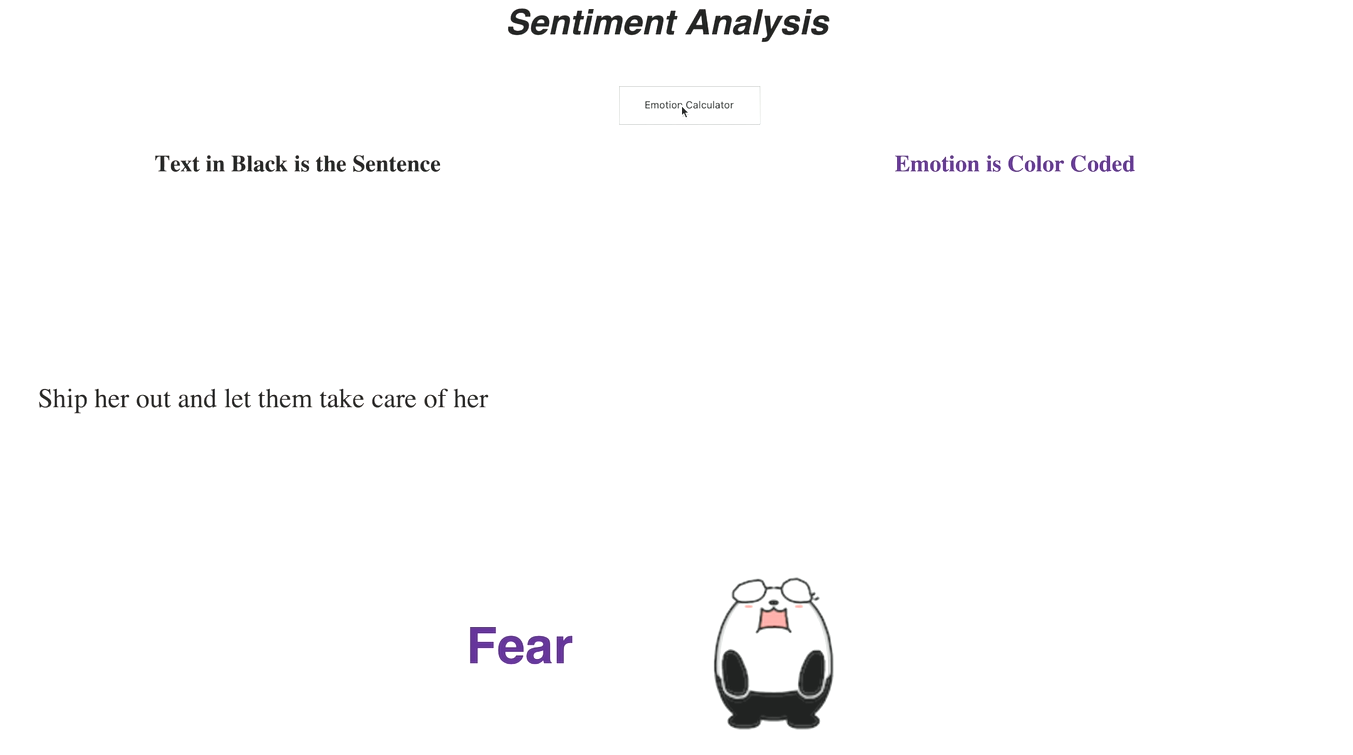
\includegraphics[scale=0.5]{images/fear.png}
\end{figure}

\newpage
\onecolumn
Figure 4 illustrates that the model labeled the comment “I’d like to stop it too… but crooks be crooks” as Sadness.

\begin{figure}[H]
\label{fig:sad}
\caption{Example of Sadness Output}
\centering
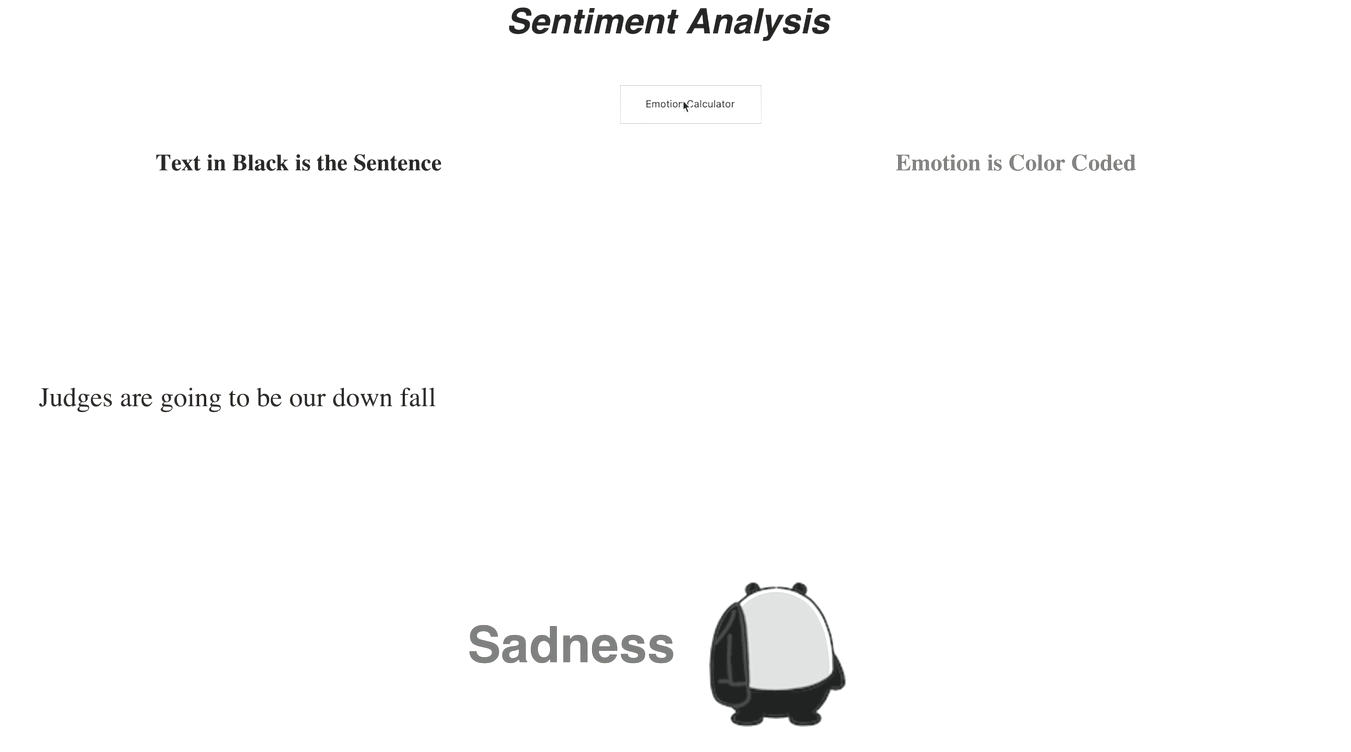
\includegraphics[scale=0.5]{images/sadness.png}
\end{figure}

\newpage
\onecolumn
Figure 5 depicts that the model labeled the comment “LOVE OUR PRESIDENT….He makes me proud again after 8 years of a DISASTER!!!” as Joy. 

\begin{figure}[H]
\label{fig:joy}
\caption{Example of Joy Output}
\centering
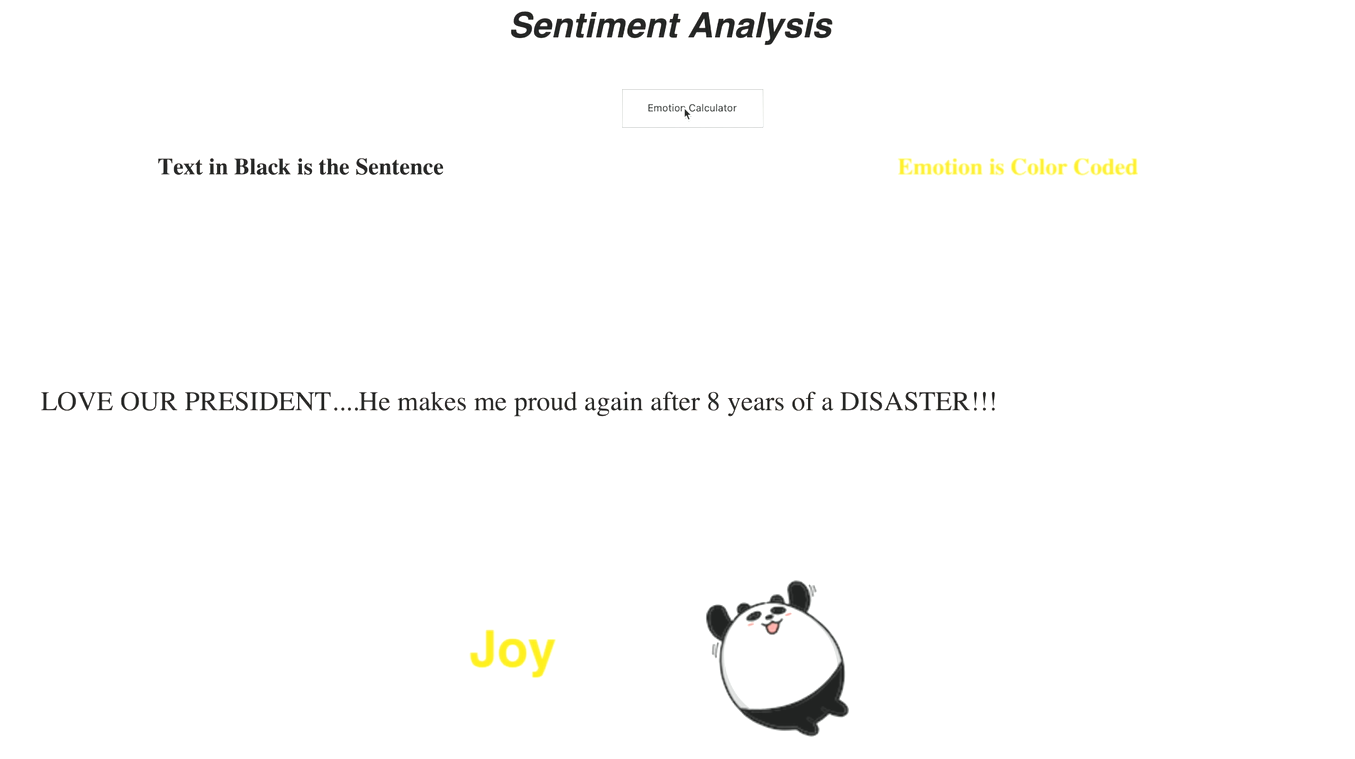
\includegraphics[scale=0.5]{images/joy.png}
\end{figure}


\end{document}
